% Provenance (never printed): see sources/outline_sources.md (Year 1: field
% notebook, compass-clinometer, hand lens, sampling, polarising microscope and
% thin sections, safety). The readings of the Varden east limb are simulated
% in figdata/bachelor-1/attitude_stats.py (seed 83, errors of 3 degrees);
% problem values in the Book 3 scratch calculator calc/ch06.py.
\chapter{Field and Lab Methods I}\label{ch:b1:field-lab-methods-1}

A geologist mapping the Varden Hills carries little: a notebook, a pencil, a
satellite receiver, a compass-clinometer, a hand lens and a few sample bags.
With them she fixes where she stands, measures the \omterm{def:b1:geological-maps:attitude}{attitude} of the beds, names
the rocks, and brings back the samples that the laboratory will cut, grind and
look at through a microscope. Every number of the earlier chapters --- an
\omterm{def:b1:geological-maps:attitude}{attitude} on a map, a \omterm{def:b1:geological-maps:attitude}{dip} in a section --- began as a reading of this kind,
with its own error. This chapter describes how professionals make these
observations, and how repeated readings are averaged and their scatter turned
into an uncertainty. It ends with a season of readings on the east limb of the
Varden \omterm{def:b1:geological-maps:fold}{anticline}.

\begin{recall}
The \omterm{def:b1:geological-maps:attitude}{attitude} of a plane is written \omterm{def:b1:geological-maps:attitude}{dip direction}/\omterm{def:b1:geological-maps:attitude}{dip}, as $081/12$, or as a
\omterm{def:b1:geological-maps:attitude}{strike} by the right-hand rule with a \omterm{def:b1:geological-maps:attitude}{dip} (\cref{ch:b1:geological-maps}). The
magnetic declination is the angle between geographic north and the direction
in which a compass needle points (physics, grade 11). Minerals are recognised
in the hand by their lustre, cleavage, hardness and colour (Book 2, grade 11).
The mean and the standard deviation of a set of numbers summarise their centre
and their scatter (mathematics).
\end{recall}

\section{The notebook and the map}

\begin{definition}[Field station, field notebook]\label{def:b1:field-lab-methods-1:station}
A \emph{field station}\index{field station} is a numbered place where a
geologist makes and records observations: its position, the rocks seen, their
\omterm{def:b1:geological-maps:attitude}{attitude}, and the samples taken. The \emph{field notebook}\index{field
notebook} is the bound record of the stations, in the order they were visited,
with their numbers, sketches and measurements, written on the spot.
\end{definition}

The notebook is the primary record: what is not written at the station is
lost, and a map drawn in the evening is only as good as the notes behind it.
Each station has a number that appears on the field map, in the notebook, and
on every sample bag taken there. A sketch shows what a list of numbers cannot
--- how two units meet, which way younger beds lie, where a reading was taken
on a folded surface --- and records its scale and orientation. Facts and
interpretations are kept apart: ``limestone on shale, contact sharp'' is an
observation; ``\omterm{def:b1:cross-sections:unconformity}{unconformity}'' is an inference, written as such.

\begin{inthefield}[A day of mapping]
% ledger: gps:smartphone-accuracy, gps:high-end
\begin{minipage}[t]{0.58\linewidth}\vspace{0pt}
A mapping geologist plans a traverse across the \omterm{def:b1:geological-maps:attitude}{strike}, so as to meet every
unit in turn, and stops wherever a contact, a change of rock or a measurable
surface appears. At each station she writes the station number and the
position, sketches what she sees, measures \omterm{def:b1:geological-maps:attitude}{attitudes}, and notes the samples.
Positions come from a satellite receiver: an ordinary receiver, such as a
smartphone's, is typically accurate to within about \qty{4.9}{m} under open
sky, worse near cliffs and trees, while survey receivers using two frequencies
or correction services reach a few centimetres. At a map scale of 1:10\,000,
\qty{4.9}{m} is half a millimetre: an ordinary receiver is good enough for
mapping, but not for measuring the slow motion of the ground
(\cref{ch:b1:plate-kinematics}).
\end{minipage}\hfill
\begin{minipage}[t]{0.39\linewidth}\vspace{0pt}
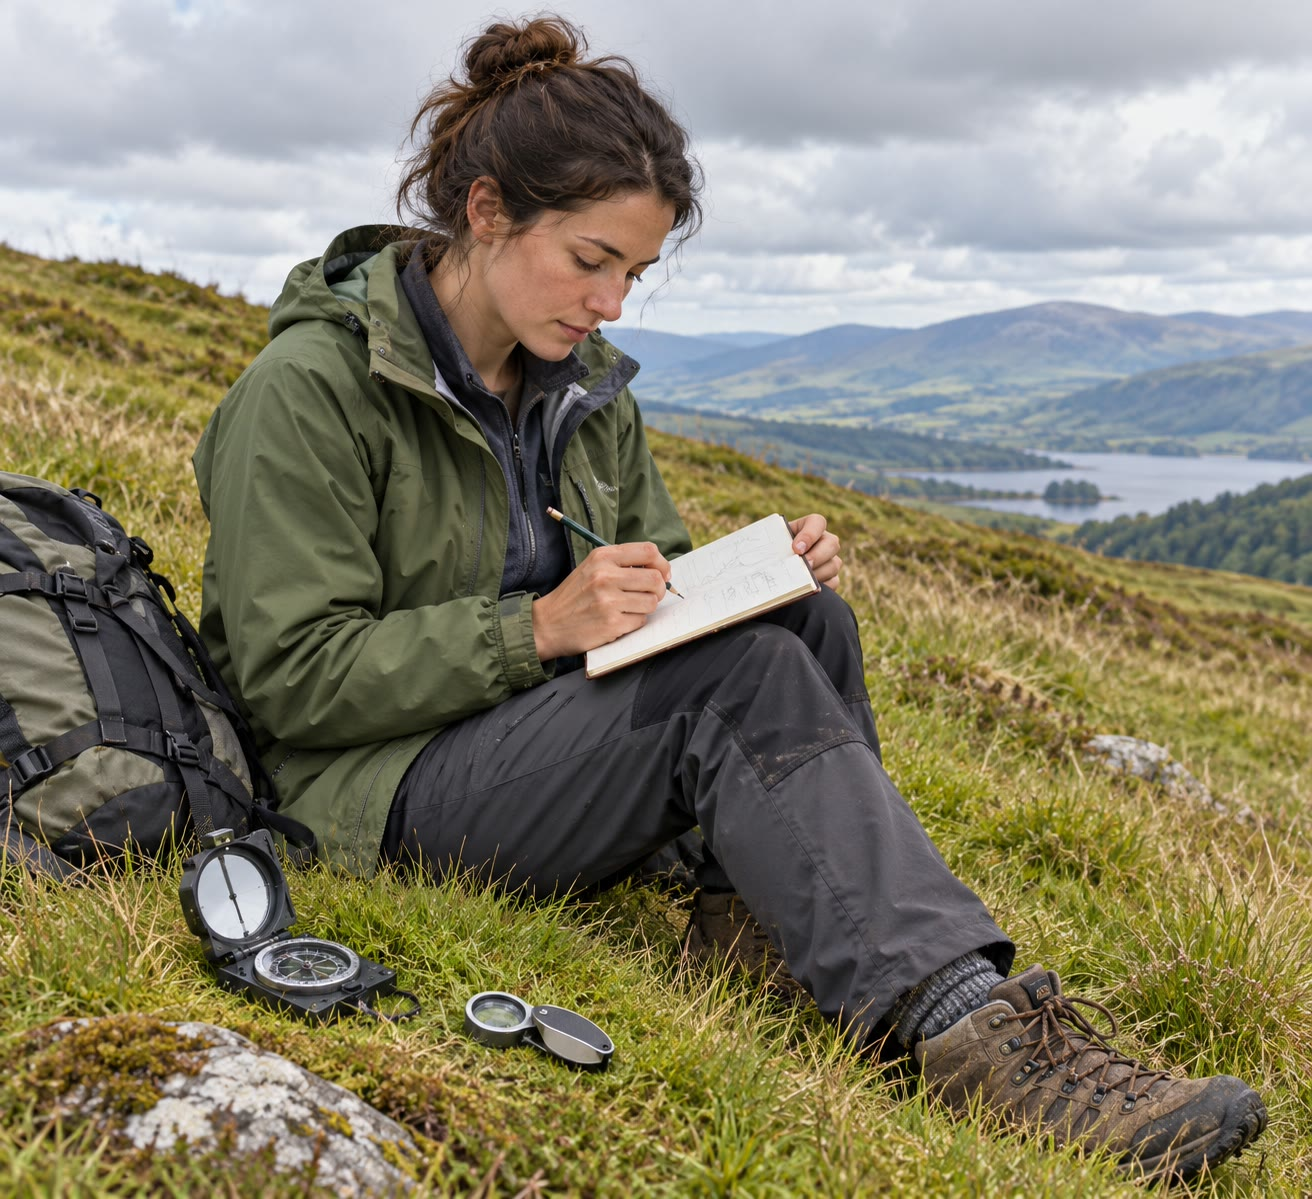
\includegraphics[width=\linewidth]{images/book3/ai/b1-field-notebook.jpg}
\end{minipage}
\end{inthefield}

\section{Measuring orientations}

The \omterm{def:b1:geological-maps:attitude}{attitude} of a plane --- a bed, a fault, a joint --- is measured with a
compass-clinometer: a magnetic compass to read \omterm{def:b1:spherical-astronomy:horizontal}{azimuths}, and a pendulum or
level to read angles from the horizontal. Its edge is laid along the \omterm{def:b1:geological-maps:attitude}{strike}
of the surface to read the \omterm{def:b1:geological-maps:attitude}{strike}, or the instrument is set on the surface
along its steepest line to read the \omterm{def:b1:geological-maps:attitude}{dip} and, from the \omterm{def:b1:spherical-astronomy:horizontal}{azimuth} of that line,
the \omterm{def:b1:geological-maps:attitude}{dip direction}.

\begin{omfigure}
\begin{tikzpicture}[font=\scriptsize]
% (a) plan view
\begin{scope}
\fill[icsJurassic!25] (0,0) -- (3.6,0.5) -- (3.9,2.9) -- (0.3,2.4) -- cycle;
\draw (0,0) -- (3.6,0.5) -- (3.9,2.9) -- (0.3,2.4) -- cycle;
\draw[omDef, thick] (0.4,1.55) -- (3.5,1.98);
\node[omDef, above, rotate=8, fill=icsJurassic!25, inner sep=1pt] at (0.95,1.65) {strike line};
% compass box laid along the strike line
\begin{scope}[shift={(2.5,1.84)}, rotate=8]
\draw[fill=white] (-0.6,0) rectangle (0.6,0.32);
\draw (0,0.16) circle (0.12);
\end{scope}
\draw[omThm, thick, -{Stealth[length=2mm]}] (1.6,1.71) -- (1.75,0.62);
\node[omThm, right, fill=icsJurassic!25, inner sep=1pt] at (1.78,0.85) {dip direction};
\node[below, align=center] at (1.95,-0.15) {(a) plan view: the edge of\\ the compass along the strike};
\draw[->] (4.3,1.6) -- (4.3,2.4) node[above] {N};
\end{scope}
% (b) side view, vertical section along the dip direction
\begin{scope}[xshift=5.8cm]
\fill[icsJurassic!25] (0,1.6) -- (3.6,0.2) -- (3.6,-0.3) -- (0,-0.3) -- cycle;
\draw[thick] (0,1.6) -- (3.6,0.2);
% clinometer resting on the surface
\begin{scope}[shift={(2.5,0.6278)}, rotate=-21.25]
\draw[fill=white] (-0.75,0) rectangle (0.75,0.3);
\draw (0,0.15) circle (0.11);
\draw[black!70] (0,0.15) -- ++(-68.75:0.11);
\end{scope}
% dip angle at the lower end of the surface
\coordinate (P) at (0.7,1.3278);
\draw[black!60] (P) -- ++(1.6,0) node[right] {horizontal};
\draw[omThm] ($(P)+(1.1,0)$) arc[start angle=0, end angle=-21.25, radius=1.1];
\node[omThm] at ($(P)+(0.9,-0.15)$) {$\delta$};
\node[below, align=center] at (1.8,-0.35) {(b) section along the dip direction:\\ the clinometer on the steepest line};
\end{scope}
\end{tikzpicture}

{\small Measuring an \omterm{def:b1:geological-maps:attitude}{attitude} (schematic). (a) The edge of the compass laid
horizontally on the bed gives the \omterm{def:b1:geological-maps:attitude}{strike}; the \omterm{def:b1:geological-maps:attitude}{dip direction} is perpendicular
to it, down the bed. (b) Set on its edge along the steepest line, the
clinometer gives the \omterm{def:b1:geological-maps:attitude}{dip} $\delta$.}
\end{omfigure}

A line --- a \omterm{def:b1:geological-maps:fold}{fold axis}, a scratch on a fault surface, the long axis of
pebbles --- has an orientation of its own.

\begin{definition}[Trend and plunge]\label{def:b1:field-lab-methods-1:trend-plunge}
The \emph{trend}\index{trend (of a line)} of a line is the \omterm{def:b1:spherical-astronomy:horizontal}{azimuth} of its
horizontal projection, measured toward the end of the line that points
downward. Its \emph{plunge}\index{plunge} is the angle between the line and
the horizontal, measured in the vertical plane that contains it. A line
plunging \ang{20} toward \ang{015} is written $20\to015$.
\end{definition}

A line of \omterm{def:b1:field-lab-methods-1:trend-plunge}{trend} $t$ and \omterm{def:b1:field-lab-methods-1:trend-plunge}{plunge} $p$ has the downward unit vector
$(\cos p\sin t, \cos p\cos t, -\sin p)$ in east, north and up components;
a line lying in a plane of \omterm{def:b1:geological-maps:attitude}{dip direction} $\alpha$ and \omterm{def:b1:geological-maps:attitude}{dip} $\delta$ \omterm{def:b1:field-lab-methods-1:trend-plunge}{plunges} by
the \omterm{def:b1:cross-sections:apparent-dip}{apparent dip} of that plane in the vertical plane of \omterm{def:b1:spherical-astronomy:horizontal}{azimuth} $t$, so that
$\tan p = \tan\delta\cos(\alpha - t)$ (\cref{thm:b1:cross-sections:apparent-dip}).

\subsection{The magnetic declination}

A compass needle points to magnetic north, not to geographic north; the angle
between the two is the magnetic declination, counted positive when magnetic
north lies east of geographic north. Maps and the \omterm{def:b1:geological-maps:attitude}{attitudes} of this book use
geographic \omterm{def:b1:spherical-astronomy:horizontal}{azimuths}.

\begin{method}[Correcting a compass azimuth]\label{met:b1:field-lab-methods-1:declination}
\begin{enumerate}
  \item Find the magnetic declination $D$ for the place and the date, from a
        model of the Earth's field (east positive, west negative).
  \item Add it to every \omterm{def:b1:spherical-astronomy:horizontal}{azimuth} read on the compass: geographic \omterm{def:b1:spherical-astronomy:horizontal}{azimuth} $=$
        magnetic \omterm{def:b1:spherical-astronomy:horizontal}{azimuth} $+ D$, taken modulo \ang{360}.
  \item Leave \omterm{def:b1:geological-maps:attitude}{dips} and \omterm{def:b1:field-lab-methods-1:trend-plunge}{plunges} alone: they are measured from the horizontal,
        with gravity, not with the needle.
\end{enumerate}
Most field compasses can be set to add $D$ mechanically; the setting, and the
year it was made for, are written in the notebook.
\end{method}

\begin{dated}{2026}
% ledger: noaa:wmm-edinburgh, noaa:wmm-reykjavik, noaa:wmm-anchorage, noaa:wmm-wellington
On 1 January 2026, the World Magnetic Model (version 2025) gives the
magnetic declination as \ang{-0.47} (west) at Edinburgh, changing by
\ang{+0.20} a year; \ang{-11.28} at Reykjavik, changing by \ang{+0.30} a year;
\ang{+14.20} (east) at Anchorage, changing by \ang{-0.28} a year; and
\ang{+23.23} at Wellington. A geologist who forgot the correction at
Wellington would misplace every \omterm{def:b1:spherical-astronomy:horizontal}{azimuth} by more than \ang{23}; one who reused
an Edinburgh setting from ten years before would carry an error of about
\ang{2}.
\end{dated}

\subsection{Repeated readings}

A single reading of a bedding plane carries errors: the surface is never a
perfect plane, the instrument is not perfectly set, and the reading is rounded
to the degree. A geologist therefore measures the same surface several times,
or several surfaces of the same limb, and averages. Averaging \omterm{def:b1:spherical-astronomy:horizontal}{azimuths} needs
care: the readings \ang{355} and \ang{005} describe directions \ang{10} apart,
but their arithmetic mean, \ang{180}, points the opposite way. The right mean
works with vectors.

\begin{definition}[Mean orientation (vector mean)]\label{def:b1:field-lab-methods-1:mean-orientation}
For a plane of \omterm{def:b1:geological-maps:attitude}{dip direction} $\alpha$ and \omterm{def:b1:geological-maps:attitude}{dip} $\delta$, let
\[
  \vec n = (\sin\delta\sin\alpha,\ \sin\delta\cos\alpha,\ \cos\delta)
\]
be its upward unit normal in east, north and up components. The \emph{mean
orientation}\index{mean orientation} (or \emph{vector mean}) of $N$ readings
of normals $\vec n_1, \dots, \vec n_N$ is the plane whose normal is
$\vec m = \vec S/\|\vec S\|$, where $\vec S = \sum_i \vec n_i$ is their
resultant; $\bar R = \|\vec S\|/N$ is the \emph{mean resultant length}. The
mean \omterm{def:b1:geological-maps:attitude}{dip direction} and \omterm{def:b1:geological-maps:attitude}{dip} are $\bar\alpha = \operatorname{atan2}(S_E, S_N)$
and $\bar\delta = \arccos(S_U/\|\vec S\|)$.
\end{definition}

That $\vec n$ is the normal follows from \cref{ch:b1:geological-maps}: the
plane $z = -\tan\delta\,(x\sin\alpha + y\cos\alpha)$ has the upward normal
$(\tan\delta\sin\alpha, \tan\delta\cos\alpha, 1)$, whose length is
$1/\cos\delta$.

\begin{proposition}[The vector mean is the closest direction]\label{prop:b1:field-lab-methods-1:vector-mean}
Among all unit vectors $\vec u$, the mean normal $\vec m$ maximises
$\sum_i \vec n_i\cdot\vec u = \sum_i \cos\theta_i(\vec u)$, where
$\theta_i(\vec u)$ is the angle between $\vec n_i$ and $\vec u$; equivalently,
it minimises $\sum_i \|\vec n_i - \vec u\|^2$. Moreover
\[
  \bar R = \frac1N\sum_i \cos\theta_i, \qquad \theta_i = \theta_i(\vec m),
\]
so that $0 < \bar R \le 1$, with $\bar R = 1$ only if all readings agree, and,
when the scatter is small, the root-mean-square angle between the readings and
their mean is
\[
  \theta_{\text{rms}} \approx \sqrt{2(1 - \bar R)} \quad\text{(radians)}.
\]
\end{proposition}

\begin{proof}
$\sum_i \vec n_i\cdot\vec u = \vec S\cdot\vec u \le \|\vec S\|$ by the
Cauchy--Schwarz inequality, with equality exactly when $\vec u = \vec m$.
Since $\|\vec n_i - \vec u\|^2 = 2 - 2\,\vec n_i\cdot\vec u$, the two problems
are the same. With $\vec u = \vec m$ the bound is reached:
$\|\vec S\| = \sum_i\cos\theta_i$, which is the formula for $\bar R$. Finally
$\cos\theta \approx 1 - \theta^2/2$ for small $\theta$, so $1 - \bar R \approx
\frac1N\sum_i\theta_i^2/2 = \theta_{\text{rms}}^2/2$.
\end{proof}

How do errors in the two angles move the normal? Differentiating $\vec n$,
\[
  \frac{\partial\vec n}{\partial\delta} = (\cos\delta\sin\alpha,\ \cos\delta\cos\alpha,\ -\sin\delta),
  \qquad
  \frac{\partial\vec n}{\partial\alpha} = (\sin\delta\cos\alpha,\ -\sin\delta\sin\alpha,\ 0):
\]
the first has length 1, the second length $\sin\delta$, and the two are
perpendicular. Small errors $\Delta\delta$ and $\Delta\alpha$ therefore
turn the normal by the angle
\[
  \Delta\theta \approx \sqrt{\Delta\delta^2 + \sin^2\delta\,\Delta\alpha^2}.
\]
On a gently dipping bed an error in the \omterm{def:b1:geological-maps:attitude}{dip direction} hardly changes the
plane: on a bed dipping \ang{12}, a \ang{3} error in \omterm{def:b1:geological-maps:attitude}{dip direction} turns the
plane by only $3\sin\ang{12} = \ang{0.6}$. The converse is the field
geologist's difficulty: the \omterm{def:b1:geological-maps:attitude}{dip direction} of a gentle bed is poorly fixed by
its plane, and small undulations of the surface scatter it widely. The
standard error of a mean of $N$ independent readings of standard deviation
$s$ is $s/\sqrt N$ (mathematics): to halve it, four times as many readings
are needed.

\begin{omfigure}
\begin{tikzpicture}
\begin{axis}[name=dd, width=0.47\linewidth, height=4.6cm, ybar, bar width=0.8,
  xmin=72.5, xmax=88.5, ymin=0, ymax=8.5, ytick={0,2,4,6,8},
  tick label style={font=\scriptsize}, label style={font=\small},
  xlabel={dip direction (\si{\degree})}, ylabel={readings}]
\addplot[fill=icsJurassic!40, draw=black] table[x=value, y=count] {figdata/out/bachelor-1-attitude_stats-hist-dd.dat};
\draw[omThm, thick] (axis cs:80.84,0) -- (axis cs:80.84,8.5);
\draw[omThm, densely dashed] (axis cs:77.91,0) -- (axis cs:77.91,8.5);
\draw[omThm, densely dashed] (axis cs:83.77,0) -- (axis cs:83.77,8.5);
\end{axis}
\begin{axis}[at={(dd.east)}, anchor=west, xshift=1.1cm, width=0.47\linewidth, height=4.6cm,
  ybar, bar width=0.8, xmin=5.5, xmax=18.5, ymin=0, ymax=8.5, ytick={0,2,4,6,8},
  tick label style={font=\scriptsize}, label style={font=\small},
  xlabel={dip (\si{\degree})}]
\addplot[fill=icsJurassic!40, draw=black] table[x=value, y=count] {figdata/out/bachelor-1-attitude_stats-hist-dip.dat};
\draw[omThm, thick] (axis cs:12.36,0) -- (axis cs:12.36,8.5);
\draw[omThm, densely dashed] (axis cs:10.24,0) -- (axis cs:10.24,8.5);
\draw[omThm, densely dashed] (axis cs:14.48,0) -- (axis cs:14.48,8.5);
\end{axis}
\end{tikzpicture}

{\small Twenty-five simulated readings of the bedding of the Varden east limb,
whose model \omterm{def:b1:geological-maps:attitude}{attitude} is $080.7/12.2$, each with errors of \ang{3} standard
deviation on both angles, rounded to the degree. Solid line: the mean; dashed:
one standard deviation either side ($080.8 \pm 2.9$ and $12.4 \pm 2.1$). The
vector mean of the 25 readings is $080.9/12.3$.}
\end{omfigure}

\section{The hand lens and field identification}

Most rocks are named in the field, before any laboratory work, from the
minerals a hand lens shows and from the way the rock breaks. The geologist
looks at a fresh surface, since weathering coats and discolours the rock, and
notes the size of the grains (whether they can be seen with the naked eye,
with the lens, or not at all), their shapes, whether they interlock like a
mosaic or are cemented like sand, and any alignment. The minerals are
recognised by the properties recalled at the start of the chapter: the glassy
lustre and absence of cleavage of quartz, the two cleavages and dull
whiteness of feldspar, the flakes of mica, the rhombic cleavage of calcite.
Hardness is tried against a steel point: quartz is harder than steel and
calcite much softer.

Professionals carry a small dropper bottle of dilute hydrochloric acid: a
carbonate rock releases bubbles of carbon dioxide where the drop falls
(chemistry). Calcite reacts briskly; dolomite reacts weakly unless powdered.
The acid is handled with gloves and eye protection, and never by a reader of
this book: the description is of professional practice.

\section{Samples}

\begin{definition}[Oriented sample]\label{def:b1:field-lab-methods-1:sample}
An \emph{oriented sample}\index{oriented sample} is a rock sample on which the
geologist has marked, before removing it, the \omterm{def:b1:geological-maps:attitude}{attitude} of one of its surfaces
(a \omterm{def:b1:geological-maps:attitude}{strike} line and a \omterm{def:b1:geological-maps:attitude}{dip} arrow, or the \omterm{def:b1:field-lab-methods-1:trend-plunge}{trend} of a line), so that the sample
can be put back in its field position in the laboratory.
\end{definition}

A sample is useful only if it is representative of the unit it stands for ---
fresh, not weathered, not taken from a vein or a fallen block --- and if its
origin is certain. Each one receives the station number and a sample number,
written on the rock and on the bag, and is listed in the notebook with its
position, its unit and the reason it was taken. Samples for chemical or
isotopic analysis, whose results may be published decades later, are tracked
from the field to the laboratory by a written record of every hand they pass
through --- a chain of custody --- so that no doubt remains about which rock
gave which number. \omterm{def:b1:field-lab-methods-1:sample}{Oriented samples} are needed whenever the direction of
something inside the rock matters: an alignment of minerals, a fabric seen
under the microscope, or the direction of the magnetisation the rock
acquired when it formed.

\section{Thin sections and the polarising microscope}

\begin{definition}[Thin section]\label{def:b1:field-lab-methods-1:thin-section}
A \emph{thin section}\index{thin section} is a slice of rock, glued to a
glass slide and ground to a standard thickness of \qty{30}{\micro\metre}, thin
enough for most minerals to transmit light.
\end{definition}

\begin{inthelab}[Making a thin section]
% ledger: jaic:thin-section, jaic:epoxy-ri
\begin{minipage}[t]{0.58\linewidth}\vspace{0pt}
In the preparation laboratory, a technician cuts a small block from the
sample with a diamond saw, grinds one face perfectly flat, and glues it to a
glass slide with an epoxy resin whose refractive index, 1.54 to 1.55, is
almost that of quartz. Most of the block is then sawn off, and the slice is
ground down on a rotating lap with ever finer abrasive until it is
\qty{30}{\micro\metre} thick. The technician checks the thickness under the
microscope from the colours shown by quartz grains (\cref{ch:b1:optical-mineralogy}),
and finishes with a thin cover glass or a polished surface. Porous or crumbly
rocks are first soaked in resin so that they hold together.
\end{minipage}\hfill
\begin{minipage}[t]{0.39\linewidth}\vspace{0pt}
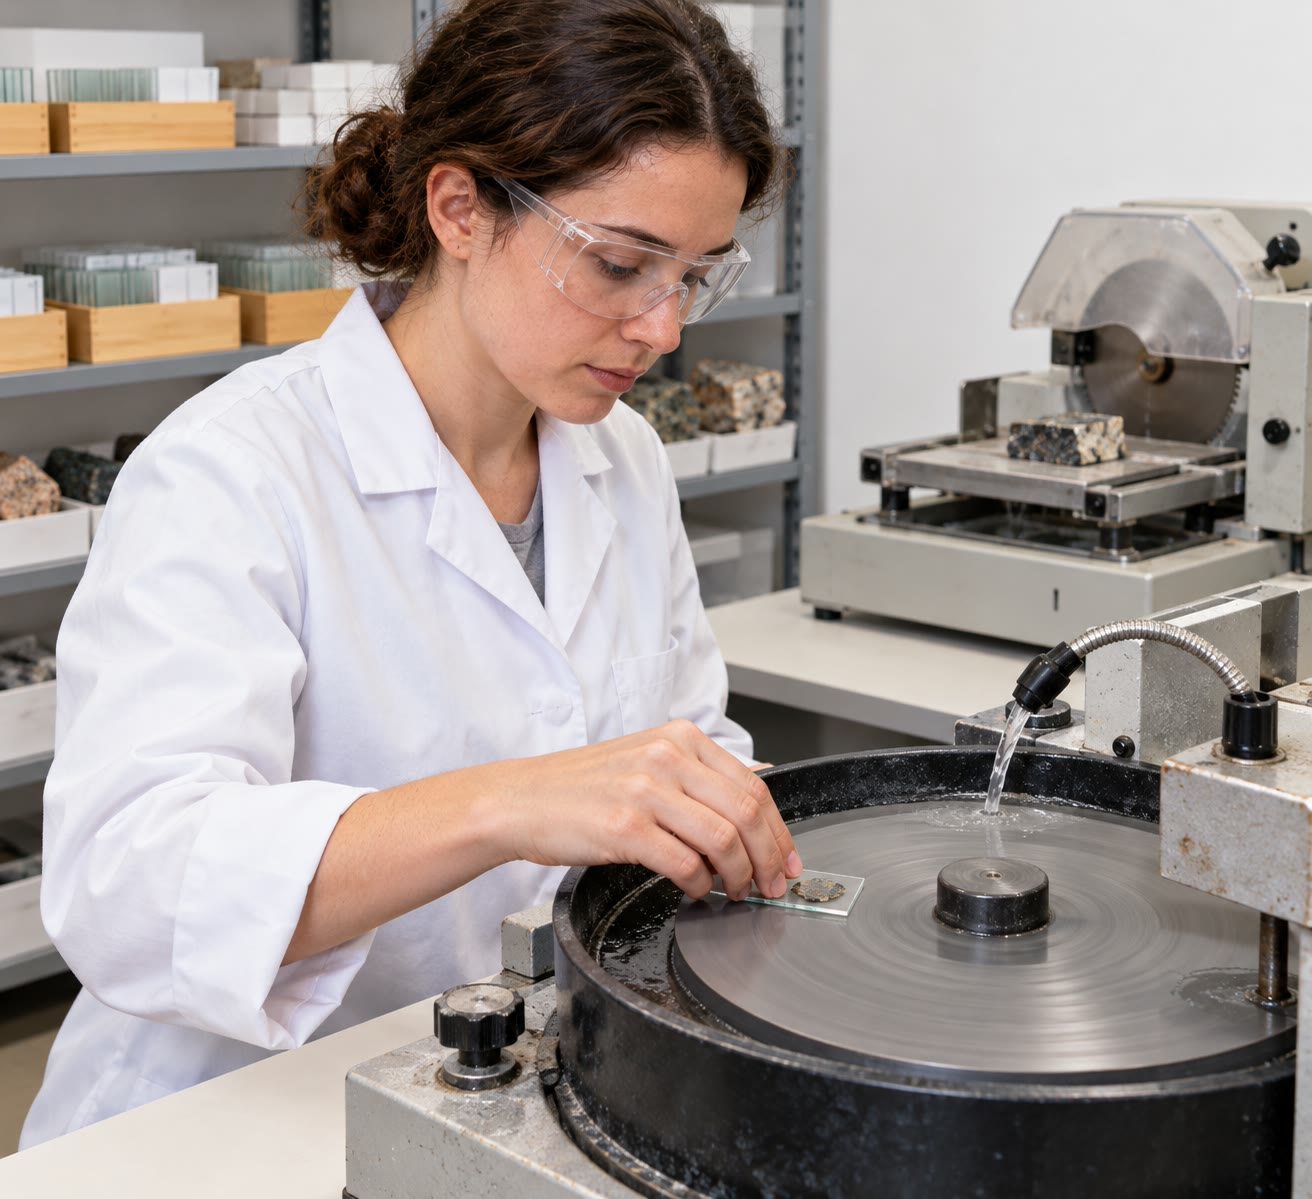
\includegraphics[width=\linewidth]{images/book3/ai/b1-thin-section-lab.jpg}
\end{minipage}
\end{inthelab}

The \omterm{def:b1:field-lab-methods-1:thin-section}{thin section} is studied with a microscope fitted with two polarising
filters. Linear polarisation is the subject of physics: here it is enough
that a polarising filter transmits only light vibrating in one direction, and
that two filters set at right angles transmit nothing.

\begin{definition}[Polarising microscope, plane-polarised light, crossed polars]\label{def:b1:field-lab-methods-1:microscope}
A \emph{polarising microscope}\index{polarising microscope} is a transmitted
light microscope with a polarising filter (the polariser) below a stage that
rotates through \ang{360} against a graduated scale, and a second polarising
filter (the analyser) between the objective and the eyepiece, which can be
moved in or out of the light path, its vibration direction at right angles to
the polariser's. With the analyser out, the specimen is seen in
\emph{plane-polarised light}\index{plane-polarised light}; with the analyser
in, it is seen between \emph{crossed polars}\index{crossed polars}.
\end{definition}

\begin{omfigure}
\begin{tikzpicture}[font=\scriptsize, x=1cm, y=0.62cm]
\def\comp#1#2#3{\draw[fill=#3] (-1.1,#1-0.18) rectangle (1.1,#1+0.18); \node[right] at (1.3,#1) {#2};}
\draw[omThm!60, line width=3pt, -{Stealth[length=3mm]}] (0,0.3) -- (0,10.6);
\draw[fill=yellow!40] (0,0) circle (0.3); \node[right] at (1.3,0) {lamp};
\comp{1.3}{polariser: transmits one vibration direction}{omDef!25}
\draw[omDef, thick, <->] (-0.5,1.3) -- (0.5,1.3);
\draw[fill=white] (-1.0,2.3) .. controls (0,2.75) .. (1.0,2.3) .. controls (0,1.85) .. (-1.0,2.3);
\node[right] at (1.3,2.3) {condenser};
\draw[fill=black!70] (-1.6,3.4) rectangle (1.6,3.55);
\draw[fill=icsJurassic!40] (-0.5,3.55) rectangle (0.5,3.65);
\node[right] at (1.7,3.48) {rotating stage, graduated in degrees, with the thin section};
\draw[fill=white] (-0.45,4.5) rectangle (0.45,5.4); \node[right] at (1.3,4.95) {objective};
\comp{6.2}{accessory slot}{black!10}
\comp{7.2}{analyser: in (crossed polars) or out (plane-polarised light)}{omDef!25}
\draw[omDef, thick, <->] (0,6.85) -- (0,7.55);
\comp{8.2}{Bertrand lens (optional)}{black!5}
\draw[fill=white] (-0.35,9.1) rectangle (0.35,10.0); \node[right] at (1.3,9.55) {eyepiece with cross-wires};
\end{tikzpicture}

{\small The light path of a \omterm{def:b1:field-lab-methods-1:microscope}{polarising microscope} (schematic, from bottom to
top). The polariser and the analyser vibrate at right angles (double arrows);
with nothing between them, \omterm{def:b1:field-lab-methods-1:microscope}{crossed polars} give a black field.}
\end{omfigure}

Between \omterm{def:b1:field-lab-methods-1:microscope}{crossed polars}, the glass of the slide, the epoxy and any isotropic
mineral (one whose optical properties are the same in every direction, as in
cubic crystals) stay black whatever the rotation of the stage. Most minerals
are not isotropic: they change the polarisation of the light that crosses
them, and appear in interference colours that change as the stage turns and
vanish four times in a full turn. Why they do so, and how the colours and the
angles identify a mineral, is the subject of \cref{ch:b1:optical-mineralogy}.
Minerals in \omterm{def:b1:field-lab-methods-1:thin-section}{thin section} are usually examined at magnifications from about
$16\times$ to $400\times$.
% ledger: jaic:magnification

\begin{omfigure}
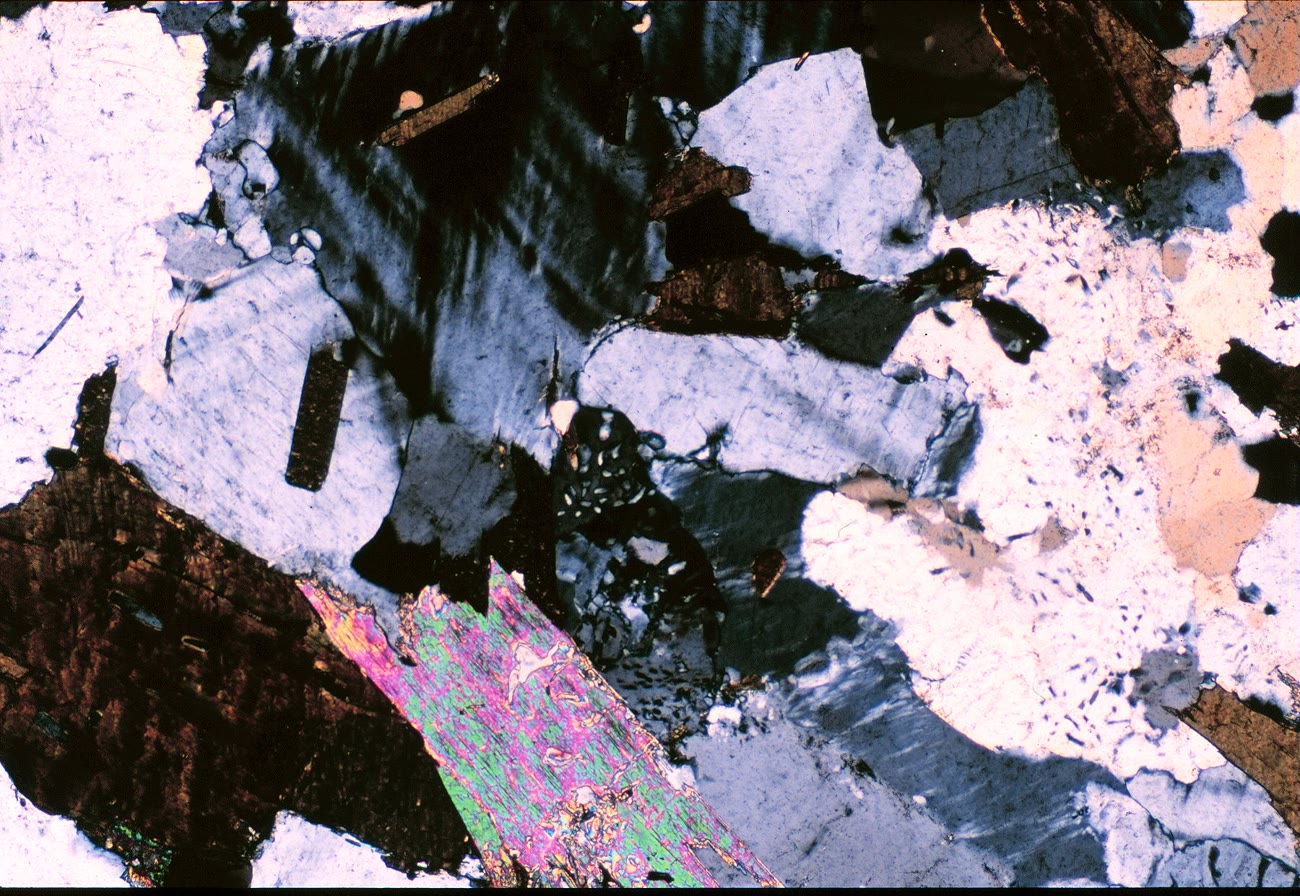
\includegraphics[width=0.55\linewidth]{images/book3/b1-granite-thin-section-xpl.jpg}
% ledger: commons:granite-xpl

{\small A granite in \omterm{def:b1:field-lab-methods-1:thin-section}{thin section} between \omterm{def:b1:field-lab-methods-1:microscope}{crossed polars}. Biotite is brown,
muscovite shows bright pink and green interference colours, plagioclase is
striped by its twinning, and quartz is white to grey. Photograph Darla
Sondrol, CC0 (Wikimedia Commons).}
\end{omfigure}

\begin{safety}
Field and laboratory work are made safe by professional rules, not by luck.
In the field, geologists work in pairs or leave a written plan of their route
and return time; they carry weather forecasts, maps and first aid, keep away
from the foot and the edge of cliffs and quarry faces, and wear a helmet and
eye protection wherever rock can fall or splinter; work on active sites
follows the operator's rules. In the laboratory, saws and laps run behind
guards with water to keep dust down, resins and acids are handled with gloves
and goggles under extraction, and every chemical has its safety data sheet.
None of these activities is for a reader of this book alone: the chapter
describes professional practice.
\end{safety}

\section{Exercises}

\begin{exercise}[$\star$]\label{exo:b1:field-lab-methods-1:1}
A satellite receiver gives positions within about \qty{4.9}{m}. How large is
that on a map at 1:10\,000? At 1:25\,000?
\end{exercise}

\begin{exercise}[$\star$]\label{exo:b1:field-lab-methods-1:2}
A compass with no declination setting reads the \omterm{def:b1:geological-maps:attitude}{dip direction} \ang{052} on a
bed. Give the geographic \omterm{def:b1:geological-maps:attitude}{dip direction} if the reading was made at Reykjavik
on 1 January 2026, then at Wellington the same day (dated box).
\end{exercise}

\begin{exercise}[$\star$]\label{exo:b1:field-lab-methods-1:3}
A \omterm{def:b1:geological-maps:fold}{fold axis} \omterm{def:b1:field-lab-methods-1:trend-plunge}{plunges} \ang{20} toward \ang{015}. Write its orientation as in the
text and give its downward unit vector in east, north and up components.
\end{exercise}

\begin{exercise}[$\star$]\label{exo:b1:field-lab-methods-1:4}
Three readings of a vertical joint give the \omterm{def:b1:spherical-astronomy:horizontal}{azimuths} of its normal \ang{350},
\ang{358} and \ang{006}. Compute their arithmetic mean, then the \omterm{def:b1:spherical-astronomy:horizontal}{azimuth} of
the sum of the three horizontal unit vectors. Which mean is right?
\end{exercise}

\begin{exercise}[$\star\star$]\label{exo:b1:field-lab-methods-1:5}
Five readings of the \omterm{def:b1:geological-maps:attitude}{dip} of one bed are \ang{34}, \ang{37}, \ang{35},
\ang{33} and \ang{36}. Compute their mean, their standard deviation and the
standard error of the mean.
\end{exercise}

\begin{exercise}[$\star\star$]\label{exo:b1:field-lab-methods-1:6}
A geologist averages one reading on each limb of a symmetric \omterm{def:b1:geological-maps:fold}{fold}: $090/30$
and $270/30$. Compute the vector mean and $\bar R$. What has gone wrong?
\end{exercise}

\begin{exercise}[$\star\star$]\label{exo:b1:field-lab-methods-1:7}
Scratches on a bedding surface of \omterm{def:b1:geological-maps:attitude}{attitude} $080/12$ have the \omterm{def:b1:field-lab-methods-1:trend-plunge}{trend}
\ang{120}. What is their \omterm{def:b1:field-lab-methods-1:trend-plunge}{plunge}? What would it be for the \omterm{def:b1:field-lab-methods-1:trend-plunge}{trend} \ang{170}?
\end{exercise}

\begin{exercise}[$\star\star$]\label{exo:b1:field-lab-methods-1:8}
At Edinburgh the magnetic declination is \ang{-0.47} on 1 January 2026 and
changes by \ang{+0.20} a year. Assuming the change stays steady, when does it
reach zero, and what is it on 1 January 2030?
\end{exercise}

\begin{exercise}[$\star\star$]\label{exo:b1:field-lab-methods-1:9}
Three readings of one bed are $080/10$, $080/12$ and $080/14$. Show that their
vector mean is $080/12$, compute $\bar R$ and the estimate
$\sqrt{2(1 - \bar R)}$ of $\theta_{\text{rms}}$, and compare with the exact
root-mean-square angle.
\end{exercise}

\begin{exercise}[$\star\star\star$]\label{exo:b1:field-lab-methods-1:10}
A \omterm{def:b1:field-lab-methods-1:thin-section}{thin section} cuts a spherical grain of radius $r$ at a distance $h$ from its
centre, with $h$ equally likely anywhere between 0 and $r$. Show that the
mean radius of the circle seen in the section is $\pi r/4$. Quartz grains
\qty{0.50}{mm} across appear on average how large in \omterm{def:b1:field-lab-methods-1:thin-section}{thin section}?
\end{exercise}

\begin{exercise}[$\star\star\star$]\label{exo:b1:field-lab-methods-1:11}
Show that if every \omterm{def:b1:geological-maps:attitude}{dip direction} of a set of readings is increased by the
same angle $D$, the \omterm{def:b1:geological-maps:attitude}{dip direction} of their vector mean increases by $D$ and
its \omterm{def:b1:geological-maps:attitude}{dip} does not change. Why does this matter for the declination correction?
\end{exercise}

\begin{exercise}[$\star\star\star$]\label{exo:b1:field-lab-methods-1:12}
On a bed dipping \ang{12}, the normal of a single reading scatters with a
standard deviation of \ang{2} in each of two perpendicular directions: along
the line of steepest \omterm{def:b1:geological-maps:attitude}{dip}, which changes the \omterm{def:b1:geological-maps:attitude}{dip}, and across it, which changes
the \omterm{def:b1:geological-maps:attitude}{dip direction}. How many readings are needed for a standard error of
\ang{0.5} on the mean \omterm{def:b1:geological-maps:attitude}{dip}? Of \ang{1} on the mean \omterm{def:b1:geological-maps:attitude}{dip direction}?
\end{exercise}

\section{Problem: A field season on the Varden east limb}

\begin{problem}[{Weekend problem --- averaging twelve compass readings, measuring
their scatter, correcting them, and comparing them with the boreholes}]
\label{pb:b1:field-lab-methods-1:1}
% readings: figdata/bachelor-1/attitude_stats.py (part normals); values: calc/ch06.py
A geologist measured the bedding of the east limb of the Varden \omterm{def:b1:geological-maps:fold}{anticline} at
twelve stations, with a compass set for the declination, rounding to the
degree. The table gives each reading (\omterm{def:b1:geological-maps:attitude}{dip direction}/\omterm{def:b1:geological-maps:attitude}{dip}) and the components of
its upward unit normal $\vec n = (n_E, n_N, n_U)$, rounded to four decimals.
\begin{center}
\small
\begin{tabular}{rcccc@{\qquad}rcccc}
\hline
 & reading & $n_E$ & $n_N$ & $n_U$ & & reading & $n_E$ & $n_N$ & $n_U$ \\
\hline
1 & $076/11$ & 0.1851 & 0.0462 & 0.9816 & 7 & $083/11$ & 0.1894 & 0.0233 & 0.9816 \\
2 & $081/13$ & 0.2222 & 0.0352 & 0.9744 & 8 & $083/12$ & 0.2064 & 0.0253 & 0.9781 \\
3 & $078/16$ & 0.2696 & 0.0573 & 0.9613 & 9 & $085/12$ & 0.2071 & 0.0181 & 0.9781 \\
4 & $081/11$ & 0.1885 & 0.0298 & 0.9816 & 10 & $078/11$ & 0.1866 & 0.0397 & 0.9816 \\
5 & $076/10$ & 0.1685 & 0.0420 & 0.9848 & 11 & $081/13$ & & & \\
6 & $083/14$ & 0.2401 & 0.0295 & 0.9703 & 12 & $082/11$ & & & \\
\hline
\end{tabular}
\end{center}

\medskip
\noindent\textbf{Part I --- The mean attitude.}
\begin{enumerate}
  \item Compute the arithmetic means of the twelve \omterm{def:b1:geological-maps:attitude}{dip directions} and of the
        twelve \omterm{def:b1:geological-maps:attitude}{dips}.
  \item Give an example of two readings for which the arithmetic mean of the
        \omterm{def:b1:geological-maps:attitude}{dip directions} is absurd, and say why it is safe here.
  \item Show that $\vec n = (\sin\delta\sin\alpha, \sin\delta\cos\alpha,
        \cos\delta)$ is a unit vector perpendicular to the \omterm{def:b1:geological-maps:attitude}{dip} line and to
        the \omterm{def:b1:geological-maps:attitude}{strike} line of the plane $\alpha/\delta$.
  \item Complete the table for readings 11 and 12.
  \item Compute the resultant $\vec S$ of the twelve normals.
  \item Compute $\|\vec S\|$ and the mean resultant length $\bar R$.
  \item Deduce the vector mean: its \omterm{def:b1:geological-maps:attitude}{dip direction} and its \omterm{def:b1:geological-maps:attitude}{dip}.
\end{enumerate}

\medskip
\noindent\textbf{Part II --- The scatter.}
\begin{enumerate}[resume]
  \item Compute the sample standard deviations of the \omterm{def:b1:geological-maps:attitude}{dip directions} and of
        the \omterm{def:b1:geological-maps:attitude}{dips}.
  \item Using \cref{prop:b1:field-lab-methods-1:vector-mean}, estimate the
        root-mean-square angle $\theta_{\text{rms}}$ between the readings and
        their mean, in degrees.
  \item Predict $\theta_{\text{rms}}$ from the two standard deviations of
        question 8 and the error formula of the chapter, and compare.
  \item Which of the two standard deviations contributes most to
        $\theta_{\text{rms}}$, and why?
  \item Compute the standard errors of the mean \omterm{def:b1:geological-maps:attitude}{dip} and of the mean \omterm{def:b1:geological-maps:attitude}{dip
        direction}.
  \item Is the scatter of the \omterm{def:b1:geological-maps:attitude}{dip directions}, \ang{2.9}, a sign of careless
        measurement? Explain.
\end{enumerate}

\medskip
\noindent\textbf{Part III --- The declination.}
\begin{enumerate}[resume]
  \item A second geologist forgot to set the declination. Her twelve readings
        have the vector mean $083.1/12.1$ in magnetic \omterm{def:b1:spherical-astronomy:horizontal}{azimuths}. Suppose the
        magnetic declination in the Varden Hills that year is \ang{2.5} west.
        What is her mean in geographic \omterm{def:b1:spherical-astronomy:horizontal}{azimuths}?
  \item Why is her mean \omterm{def:b1:geological-maps:attitude}{dip} right without correction?
  \item Could she have corrected each reading before averaging, rather than
        the mean? Does it change the answer (\cref{exo:b1:field-lab-methods-1:11})?
  \item Ten years later, a student reuses her declination setting while the
        declination has changed by \ang{0.2} a year. How large is the error,
        compared with the standard error of question 12?
  \item Give the \omterm{def:b1:geological-maps:attitude}{strike} of the mean \omterm{def:b1:geological-maps:attitude}{attitude} of the first geologist by the
        right-hand rule.
\end{enumerate}

\medskip
\noindent\textbf{Part IV --- Compass and boreholes.}
\begin{enumerate}[resume]
  \item From three boreholes, \cref{ch:b1:geological-maps} found the \omterm{def:b1:geological-maps:attitude}{attitude}
        $080.6/12.2$ for the base of the limestone. Compare it with the vector
        mean of question 7, angle by angle.
  \item Compute the angle between the two normals.
  \item The standard error of the mean direction is about
        $\theta_{\text{rms}}/\sqrt N$. Is the difference of question 20
        significant?
  \item How many readings would halve that standard error?
  \item Name two errors that no number of readings would reduce.
  \item Give the mean \omterm{def:b1:geological-maps:attitude}{attitude} of the east limb from the twelve readings, in
        the form \omterm{def:b1:geological-maps:attitude}{dip direction}/\omterm{def:b1:geological-maps:attitude}{dip} rounded to the degree.
\end{enumerate}
\end{problem}
